\section{Results}
\begin{table*}[t]
\caption{Synthetic primary results over ten matched seeds. Accuracy is percent; forgetting is percentage points. Values show mean $\pm$ sample SD.}
\label{tab:synthetic}
\centering\small
\begin{tabular}{llrrr}\toprule Scenario & Policy & Accuracy (\%) & Experts & Forgetting (pp)\\\midrule
Benign & Fixed & 94.29 $\pm$ 0.61 & 1.00 $\pm$ 0.00 & 0.42 $\pm$ 0.29 \\
Benign & Novelty & 94.09 $\pm$ 0.48 & 3.00 $\pm$ 0.00 & 0.19 $\pm$ 0.11 \\
Benign & Interference & 94.20 $\pm$ 0.54 & 3.10 $\pm$ 1.29 & 0.42 $\pm$ 0.27 \\
Benign & Dual & 94.29 $\pm$ 0.61 & 1.10 $\pm$ 0.32 & 0.42 $\pm$ 0.28 \\
\midrule
Conflicting & Fixed & 64.31 $\pm$ 0.69 & 1.00 $\pm$ 0.00 & 29.25 $\pm$ 0.74 \\
Conflicting & Novelty & 94.07 $\pm$ 0.50 & 3.00 $\pm$ 0.00 & 0.11 $\pm$ 0.15 \\
Conflicting & Interference & 94.01 $\pm$ 0.49 & 3.30 $\pm$ 0.48 & 0.15 $\pm$ 0.15 \\
Conflicting & Dual & 89.56 $\pm$ 10.04 & 2.70 $\pm$ 0.67 & 4.34 $\pm$ 9.91 \\
\midrule
Mixed & Fixed & 49.77 $\pm$ 0.35 & 1.00 $\pm$ 0.00 & 44.50 $\pm$ 0.42 \\
Mixed & Novelty & 93.91 $\pm$ 0.45 & 4.00 $\pm$ 0.00 & 0.31 $\pm$ 0.22 \\
Mixed & Interference & 94.09 $\pm$ 0.42 & 3.40 $\pm$ 0.70 & 0.47 $\pm$ 0.26 \\
Mixed & Dual & 81.03 $\pm$ 21.02 & 2.00 $\pm$ 0.00 & 13.47 $\pm$ 20.97 \\
\midrule
Hidden reversal & Fixed & 50.00 $\pm$ 0.42 & 1.00 $\pm$ 0.00 & 44.28 $\pm$ 0.82 \\
Hidden reversal & Novelty & 50.00 $\pm$ 0.42 & 1.00 $\pm$ 0.00 & 44.28 $\pm$ 0.82 \\
Hidden reversal & Interference & 50.00 $\pm$ 0.42 & 4.00 $\pm$ 0.00 & 44.28 $\pm$ 0.82 \\
Hidden reversal & Dual & 50.00 $\pm$ 0.42 & 1.00 $\pm$ 0.00 & 44.28 $\pm$ 0.82 \\
\bottomrule
\end{tabular}
\end{table*}

\subsection{Synthetic selectivity and missed learning}
Under benign synthetic shifts, Novelty allocates three experts at \(94.09\pm0.48\%\), while Dual allocates \(1.10\pm0.32\) at \(94.29\pm0.61\%\). This suppresses redundant allocation when contexts share one rule. Fixed capacity already matches Dual accuracy with one expert, so the outcome does not establish a need for adaptive control. Interference alone allocates \(3.10\pm1.29\) despite the shared rule, showing that local gradient opposition can arise without a new predictive function being necessary.

On conflicting rules, Novelty reaches \(94.07\pm0.50\%\) with three experts; Dual reaches \(89.56\pm10.04\%\) with \(2.70\pm0.67\). Its mean forgetting is 4.34 points, compared with 0.11 for Novelty. The paired accuracy difference is -4.50 points, with descriptive interval [-12.09,0.00]. Lower allocation partly reflects missed learning. The broad interval is not evidence that the methods preserve equivalent accuracy.

Mixed recurrence makes the distinction clearer: Novelty reaches \(93.91\pm0.45\%\) with four experts, while Dual uses two but reaches \(81.03\pm21.02\%\), with 13.47 points of forgetting. Two clean rules could be represented by two specialists, yet the controller does not consistently discover and preserve that decomposition. Interference-only succeeds at \(94.09\pm0.42\%\) while using \(3.40\pm0.70\) experts. No trigger dominates accuracy, allocation and cost across every synthetic setting.

All policies approach 50\% under hidden reversal. Identical observable context cannot identify which opposite rule applies. For the same input and opposite clean binary labels, any deterministic prediction is correct for exactly one rule; equal weighting yields one half. Symmetric independent noise preserves that population bound. Interference-only nevertheless fills four slots and averages 26.3 blocked requests. Capacity detects neither a missing identifier nor an appropriate inference distinction by itself.

\subsection{Prototype admission can remove trigger evidence}
In the primary Dual logs, three of twenty novel-context admissions on conflicting streams occur without expansion, across two seeds; twenty of thirty do so under mixed recurrence. Some are appropriate when rules are shared. Admission alone is therefore not a failure label. The relevant mechanism is that the gallery needs three novel windows while the expansion gate needs three consecutive joint windows with a stable candidate.

Table~\ref{tab:trace} shows an illustrative conflicting seed. At window 24 novelty and conflict are high, but interference falls below threshold at windows 25--26. The gallery admits context at 26. Later conflict exceeds threshold while novelty has vanished. This is an observed state coupling, not a causal proof that it explains every failed seed. Candidate changes, memory coverage and adaptation during the delay can also matter. It motivates the explicitly bounded Retained intervention.

\begin{table*}[t]
\caption{Illustrative primary joint-trigger trace at a conflicting change, seed 5. This failure example is selected after observing results and does not represent average performance. Windows are zero-indexed. The novelty threshold is 0.242 and the interference threshold is 0.2.}
\label{tab:trace}
\centering\small
\begin{tabular}{rrrrrr}
\toprule Window & Novelty & Interference & Joint condition & Experts & Prototypes\\\midrule
23 & 0.101 & 0.000 & False & 1 & 1 \\
24 & 5.041 & 0.964 & True & 1 & 1 \\
25 & 5.089 & 0.000 & False & 1 & 1 \\
26 & 5.078 & 0.126 & False & 1 & 2 \\
27 & 0.026 & 0.077 & False & 1 & 2 \\
28 & 0.134 & 0.708 & False & 1 & 2 \\
29 & 0.082 & 0.759 & False & 1 & 2 \\
30 & 0.072 & 0.843 & False & 1 & 2 \\
\bottomrule\end{tabular}
\end{table*}
Earlier synthetic sensitivity runs reduce persistence to one or change interference threshold. Persistence one raises Dual accuracy to 92.62\% on conflicting and 89.80\% on mixed streams, while benign allocation rises to 1.90 experts. It also changes immediate anchor registration, so this is not an isolated counter intervention. Threshold 0.4 reduces those accuracies to 80.77\% and 67.59\%. These post-observation settings are not selected as a validated winning configuration.

\begin{table*}[t]
\caption{Neural results over five matched seeds. All experts learn MNIST pixels. Remapped targets form an additional exploratory stress. Accuracy is percent; forgetting is percentage points; arrays count retained payload only.}
\label{tab:neural}
\centering\small
\begin{tabular}{llrrrrr}\toprule Stream & Policy & Accuracy (\%) & Experts & Forgetting (pp) & Array MiB & Gradient examples ($10^3$)\\\midrule
Contrast & Fixed & 93.61 $\pm$ 0.19 & 1.00 $\pm$ 0.00 & 0.01 & 1.969 & 235.90 \\
Contrast & Novelty & 91.30 $\pm$ 1.04 & 3.00 $\pm$ 0.00 & 0.47 & 2.804 & 235.90 \\
Contrast & Interference & 93.61 $\pm$ 0.19 & 1.00 $\pm$ 0.00 & 0.01 & 1.969 & 294.78 \\
Contrast & Dual & 93.61 $\pm$ 0.19 & 1.00 $\pm$ 0.00 & 0.01 & 1.969 & 294.78 \\
Contrast & Retained & 93.61 $\pm$ 0.19 & 1.00 $\pm$ 0.00 & 0.01 & 1.969 & 294.78 \\
\midrule
Permutation & Fixed & 91.95 $\pm$ 0.26 & 1.00 $\pm$ 0.00 & 0.40 & 1.969 & 235.90 \\
Permutation & Novelty & 92.00 $\pm$ 0.31 & 2.80 $\pm$ 0.45 & 0.07 & 2.720 & 235.90 \\
Permutation & Interference & 91.95 $\pm$ 0.26 & 1.00 $\pm$ 0.00 & 0.40 & 1.969 & 294.78 \\
Permutation & Dual & 91.95 $\pm$ 0.26 & 1.00 $\pm$ 0.00 & 0.40 & 1.969 & 294.78 \\
Permutation & Retained & 91.95 $\pm$ 0.26 & 1.00 $\pm$ 0.00 & 0.40 & 1.969 & 294.78 \\
\midrule
Remapped (exploratory) & Fixed & 91.78 $\pm$ 0.30 & 1.00 $\pm$ 0.00 & 0.37 & 1.969 & 235.90 \\
Remapped (exploratory) & Novelty & 92.02 $\pm$ 0.35 & 2.80 $\pm$ 0.45 & 0.03 & 2.720 & 235.90 \\
Remapped (exploratory) & Interference & 91.78 $\pm$ 0.30 & 1.00 $\pm$ 0.00 & 0.37 & 1.969 & 294.78 \\
Remapped (exploratory) & Dual & 91.78 $\pm$ 0.30 & 1.00 $\pm$ 0.00 & 0.37 & 1.969 & 294.78 \\
Remapped (exploratory) & Retained & 91.78 $\pm$ 0.30 & 1.00 $\pm$ 0.00 & 0.37 & 1.969 & 294.78 \\
\bottomrule
\end{tabular}
\end{table*}

\subsection{Neural contrast: sharing helps, but fixed capacity suffices}
On real-image contrast streams, Dual reaches \(93.61\pm0.19\%\) using one network, compared with \(91.30\pm1.04\%\) and three for Novelty. The paired Dual-minus-Novelty difference is +2.32 points, with descriptive interval [1.80,3.12]. Both allocation and accuracy favor reuse in this constructed setting. Specialized networks receive fewer total updates individually, whereas one shared model can exploit compatible information throughout the stream. This difference is a property of the compared controllers under the same observation budget.

Fixed, Interference, Dual and Retained follow identical training trajectories in all five contrast seeds. Their final accuracy and retained arrays match exactly; interference-based policies merely perform additional diagnostic gradient calculations. No three-window qualifying streak creates a specialist. Thus the evidence identifies avoidable novelty-driven growth, but provides no performance advantage for computing interference over simply maintaining fixed capacity.

\begin{figure*}[t]\centering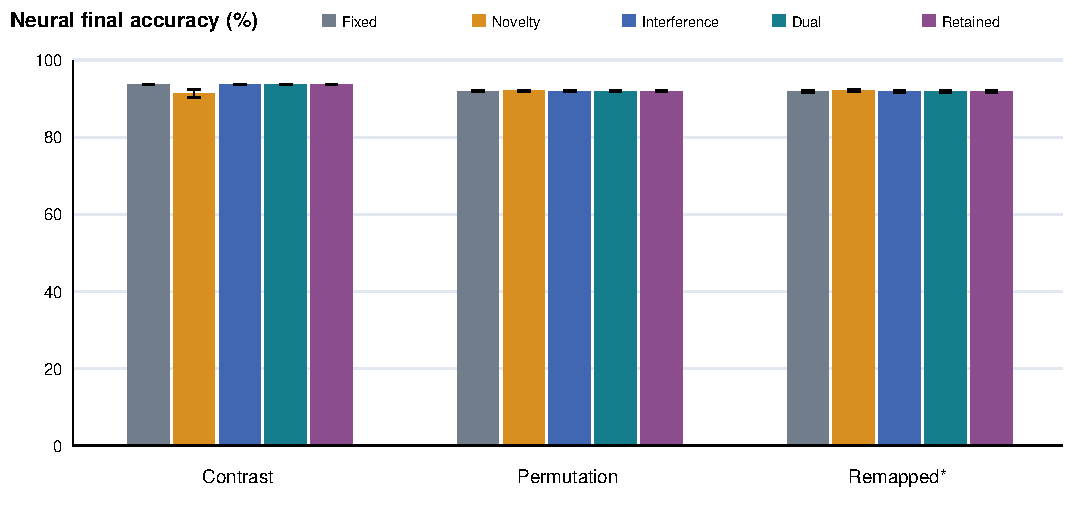
\includegraphics[width=\textwidth]{neural_accuracy.pdf}
\caption{MNIST-derived results. Bars show five-seed means and error bars show sample SD. Target remapping is an additional exploratory stress, not the ordinary digit-recognition task. Fixed, Interference, Dual and Retained overlap because their predictions match in every seed.}
\label{fig:neural_accuracy}\end{figure*}

\subsection{Neural permutation: small accuracy loss with lower allocation}
Novelty averages \(2.80\pm0.45\) networks at \(92.00\pm0.31\%\). Dual retains one at \(91.95\pm0.26\%\). Their accuracy difference is -0.047 points, with interval [-0.192,0.051]. The lower endpoint is above the neural protocol's descriptive -1-point tolerance, while allocation decreases by 1.8 networks. That satisfies the specified descriptive criterion for this stream, not a general noninferiority claim.

One Novelty seed creates only two networks. With multiple old anchors nearly equally distant from a new permuted context, the candidate can change during the three-window streak. Gallery admission can again precede allocation. Input novelty and candidate persistence therefore interact even in the nominal novelty-only baseline. Its expert count is an observed outcome rather than an assumed one-per-domain upper bound.

Fixed capacity again matches Dual. A shared two-hidden-layer network can learn multiple distinct pixel arrangements with replay at this scale. The input transformations do not establish that its representational capacity is inadequate. Slightly greater Dual forgetting, 0.40 points versus 0.07, also shows why a near-matching final mean should not conceal all retention differences.

\subsection{Exploratory target-remapping stress}
After adding incompatible domain-specific label mappings, Novelty reaches \(92.02\pm0.35\%\) with \(2.80\pm0.45\) networks. Dual reaches \(91.77\pm0.30\%\) using one. The paired difference is -0.248 points, with interval [-0.393,-0.079]. This is a small but consistently unfavorable observed difference; it should not be described as equal accuracy. It remains within the specified one-point descriptive tolerance, which is a different statement.

The fixed network still matches Dual. Distinct pixel permutations make the remapped domains distinguishable from input, and the network can represent conditional mappings. Label incompatibility alone therefore does not force growth. The stress does not demonstrate a regime where extra neural capacity is required. Because it was added after the original neural experiment started, it supplies exploratory evidence and is kept separate from the 50 initial runs.

\subsection{Retained evidence changes eligibility without improving these runs}
Retained marks two newly admitted contexts for 30 subsequent windows in each seed: 300 retained windows per stream over five seeds. It increases true gate windows from 3 to 12 on contrast, 0 to 8 on permutation, and 1 to 5 on remapping. However, none forms three consecutive conflicts with the same candidate after warm-up and cooldown. Retained therefore allocates no additional expert and exactly matches Dual predictions.

Interference exceeds 0.2 in 70 contrast, 44 permutation and 40 remapped windows across the five seeds. Isolated opposition exists, but it does not persist sufficiently for these controllers. The unit sequence establishes that Retained can change a delayed decision; the real-image experiment does not establish an accuracy or robustness gain from that change. A more difficult, independently selected setting would be needed to test that benefit rather than lowering the threshold after inspecting these test logs.

\subsection{Resource consequences depend on expert scale}
Synthetic experts occupy 24 weight-array bytes. In benign data, Dual's 1.9-expert reduction saves only 45.6 retained bytes, approximately 0.31\%; replay dominates. Joint control processes about 33\% more gradient examples. This is a weak resource trade-off despite fewer experts.

Each neural expert occupies 437,544 bytes. On contrast, Novelty retains 2.804 MiB versus 1.969 for Dual, a 29.8\% reduction. On permutation and remapping the corresponding means are 2.720 and 1.969 MiB, about 27.6\%. Replay alone occupies 1,617,920 bytes. These are meaningful retained-array differences at this model scale, but are not process-memory, peak-training or GPU-memory measurements.

Dual processes 294,780 gradient examples per neural run versus 235,904 for Novelty, approximately 25.0\% more. The fixed model achieves the same predictions and recorded storage as Dual while avoiding those diagnostic gradients. Thus larger experts change the magnitude of savings relative to Novelty without establishing that the joint controller is the most efficient available policy. CPU times are small and hardware-sensitive; no reliable deployment speedup is claimed.
